\documentclass{beamer}
\usepackage{beamerthemesplit}
\usepackage{amsmath}
\usepackage{adjustbox}
\usepackage{amssymb}
\usepackage{subfigure}
\usepackage{amsfonts}
\usepackage{newlfont}
\usepackage{graphics}
\usepackage{graphicx}
\usepackage{epsfig}
\usepackage{booktabs}
\usepackage{booktabs, longtable,array}
\usepackage{amsmath}
\usepackage[natbib=true,style=authoryear,backend=bibtex,useprefix=true]{biblatex}
\addbibresource{ref.bib}
\setbeamertemplate{headline}{}

\usepackage[english]{babel}
\usepackage[latin1]{inputenc}
%\usepackage{hyperref}
%\usepackage[round]{natbib}

% \usetheme{default}
% \usetheme{Boadilla} %# not so good
% \usetheme{Madrid} % # not so good
% \usetheme{Montpellier}
% \usetheme{Warsaw}
% \usetheme{Copenhagen}
% \usetheme{Goettingen}
% \usetheme{Hannover}
%\usetheme{Berkeley}
\usecolortheme{orchid}
\beamertemplatesolidbackgroundcolor{white!65}
\setlength{\parskip}{8pt plus 1pt minus 1pt} \setbeamertemplate{footline}[frame number]


\title[]{LOW COST HARDWARE DESIGN FOR IoT
APPLICATION IN INDUSTRIAL PROCESS}
\author{B.Tech Project Presentation Group Number-07}
\author{Gundappa DH (2015IPG-032)\\
        Kuthadi Sanjeev Kumar (2015IPG-046)\\
        Sachin Nikunj (2015IPG-78)\\
\vspace{6mm}
\textbf{Supervised by: Dr. Prasenjit Chanak}} 

\institute[]{
	
	ABV-Indian Institute of Information Technology and\\
	Management, Gwalior
}
\date{2018}


\begin{document}
	\frame{\titlepage}
	
	%\begin{frame}
	%\frametitle{Outline}
	%\tableofcontents[pausesections]
	%\end{frame}
	
	\begin{frame}\frametitle{Contents}
	\begin{itemize}
		\item	Introduction
		\item   literature review 
		\item   Objective 
		\item	Proposed scheme
		\item   Implementation 
		\item   Testing
		\item	Results
		\item   Conclusion and Future works
		\item   References
	\end{itemize}
\end{frame}
\begin{frame}\frametitle{Introduction}
\begin{itemize}
\item Internet of Things
\begin{itemize}
	\item Is a network of physical objects, embedded with sensors, electronics and software.	 
	\item Which enables network connectivity and helps in collecting and exchanging the data.	  
\end{itemize}
\item Importance
\begin{itemize}
\item The data can be shared virtually through internet. 
\item It can be next industrial revolution in terms of automation.
\end{itemize}
\end{itemize}
\end{frame}
\begin{frame}[shrink=1]{Literature Review}
\begin{center}
    \hspace{1cm}\begin{tabular}{| p{1cm} | p{2.5cm} | p{2cm} | p{5cm} |}
    \hline
    S.No & Paper Title & Author & Summary            \\
    \hline
    1 & Ultrasonic sensing system
 & \citet{steiner2018ultrasonic}
 & To avoid collision with unexpected obstacles,uses ultrasonic range finders for detection and mapping. Some of the application in present  
 \\
    \hline
    2 & Application of ultrasonic sensors in the process industry & \citet{hauptmann2002application} & Intents to systematically review applications of ultrasonic measurement techniques in the process industry, to compare these techniques with alternatives, and to present recent developments in this area.. \\
    \hline
    3  & Internet of things in industries: A survey & \citet{da2014internet}
 & Internet of Things (IoT) has provided a promising opportunity to build powerful industrial systems and applications by leveraging the growing ubiquity wireless, mobile, and sensor devices..\\
    \hline
    \end{tabular}
\end{center}
\end{frame}

\begin{frame}\frametitle{Objective}
\begin{itemize}

\item To design a multi sensor based device for data acquisition.
\item Connect different multi sensor based data acquisition board through an energy efficient communication scheme.
\item To design data acquisitions scheme to collect real life data from different deployed multi sensor based data acquisition board.
\item To design a scheme to analyze the collected data for identification of fault in the industrial machine.

\end{itemize}
\end{frame}
\begin{frame}\frametitle{Proposed scheme}

\begin{itemize}
	\item Our proposed scheme mainly work in industrial sector, to identify the machines health condition .	 
	\item When ever machines gets damaged it becomes really hard to identify the problem early but we can find some changes in sound, vibration, smoke, temperature of the machines .	 
	\item Human beings cannot identify changes sound, vibration, smoke of the machines. At this kind of situation we can use sensor to detect those changes
\end{itemize}

\end{frame}
\begin{frame}\frametitle{Proposed scheme}

\begin{itemize}
\begin{figure}[h]
\centerline{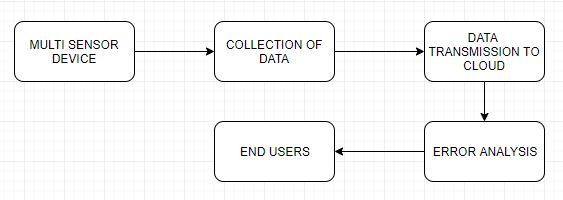
\includegraphics[width=3.7in]{SCHEME}}
\caption{Schematic diagram for proposed scheme.}
\end{figure}
	\item As the picture depict architecture of the proposed scheme, multi sensor device collect data from the monitoring field.	 
	\item Collected data gets transmit into cloud platform using the wi-fi module.	 
	\item  The collected real time is used to monitor the fault occurring in the large scale machines.
\end{itemize}

\end{frame}

\begin{frame}\frametitle{Implementation}
\item Major implementations of our objective 
\begin{itemize}
\item Integration of Multiple sensors ( Vibration sensor, smoke sensor, ultrasonic sensor, sound sensor,humidity sensor) on a micro controller embedded device.
\item Data communication between two Bluetooth modules.
\item Transmission of data to cloud platform through Wi-fi module.
\item Fault diagnosis through threshold value calculation.
\end{itemize}
\end{frame}
\begin{frame}\frametitle{Integration of multiple sensors on a micro controller embedded device}
\item Ultrasonic sensor
\begin{itemize}
\item We have used ultrasonic sensor to calculate the distance of the object placed in front of of the sensor.
\end{itemize}
\item Sound sensor
\begin{itemize}
    \item The sound sensor is used to calculate the sound variation in the surroundings.
\end{itemize}
\item Smoke  sensor
\begin{itemize}
\item Smoke sensor is used to detect a wide range of gases in the surroundings.
\item Wide range of gases include propane, butane, hydrogen etc.
\end{itemize}
\end{frame}
 \begin{frame}\frametitle{Cont'd}
 \item Vibration sensor
\begin{itemize}
    \item Vibration sensor is used to feel the vibration in the surroundings. 
    \end{itemize}
    \item Humidity and Temperature sensor
    \begin{itemize}
        \item Humidity and temperature sensor is used to calculate the relative humidity in the air.
        \item It is also used to calculate the change in the temperature in the surroundings.
    \end{itemize}
\end{frame}

\begin{frame}\frametitle{Master circuit diagram }
  \begin{figure}[H]
  \centerline{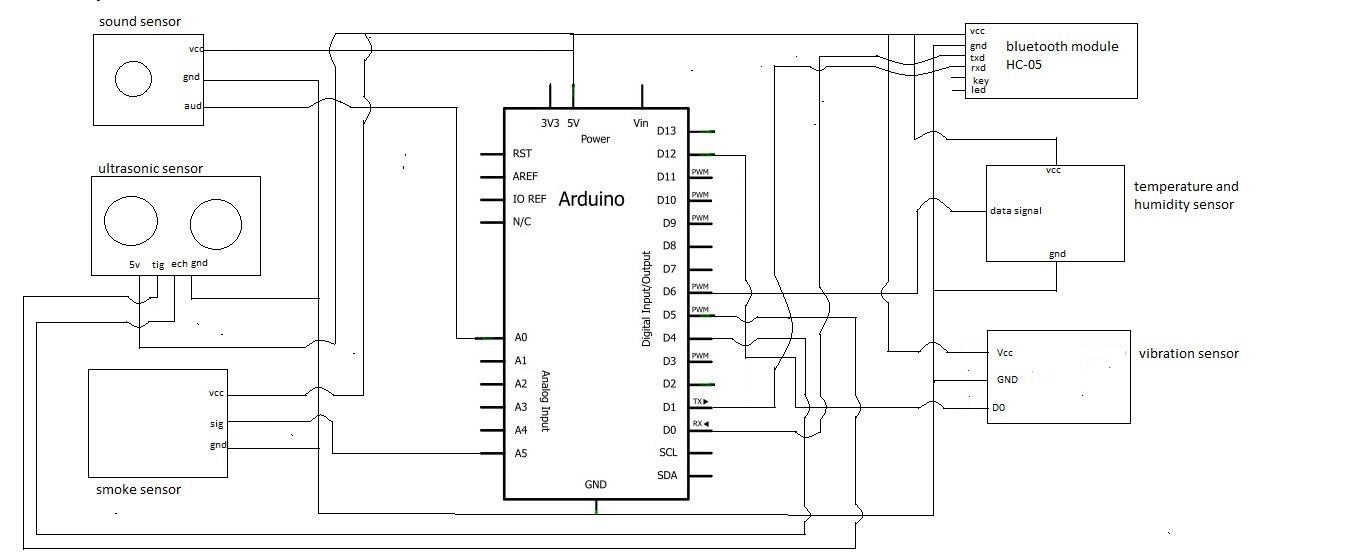
\includegraphics[width=4.0in]{MC.JPG}}
  \caption{ \textbf{}Master device circuit diagram}
  \end{figure}
\end{frame}
\begin{frame}\frametitle{Master device}
  \begin{figure}
  \centerline{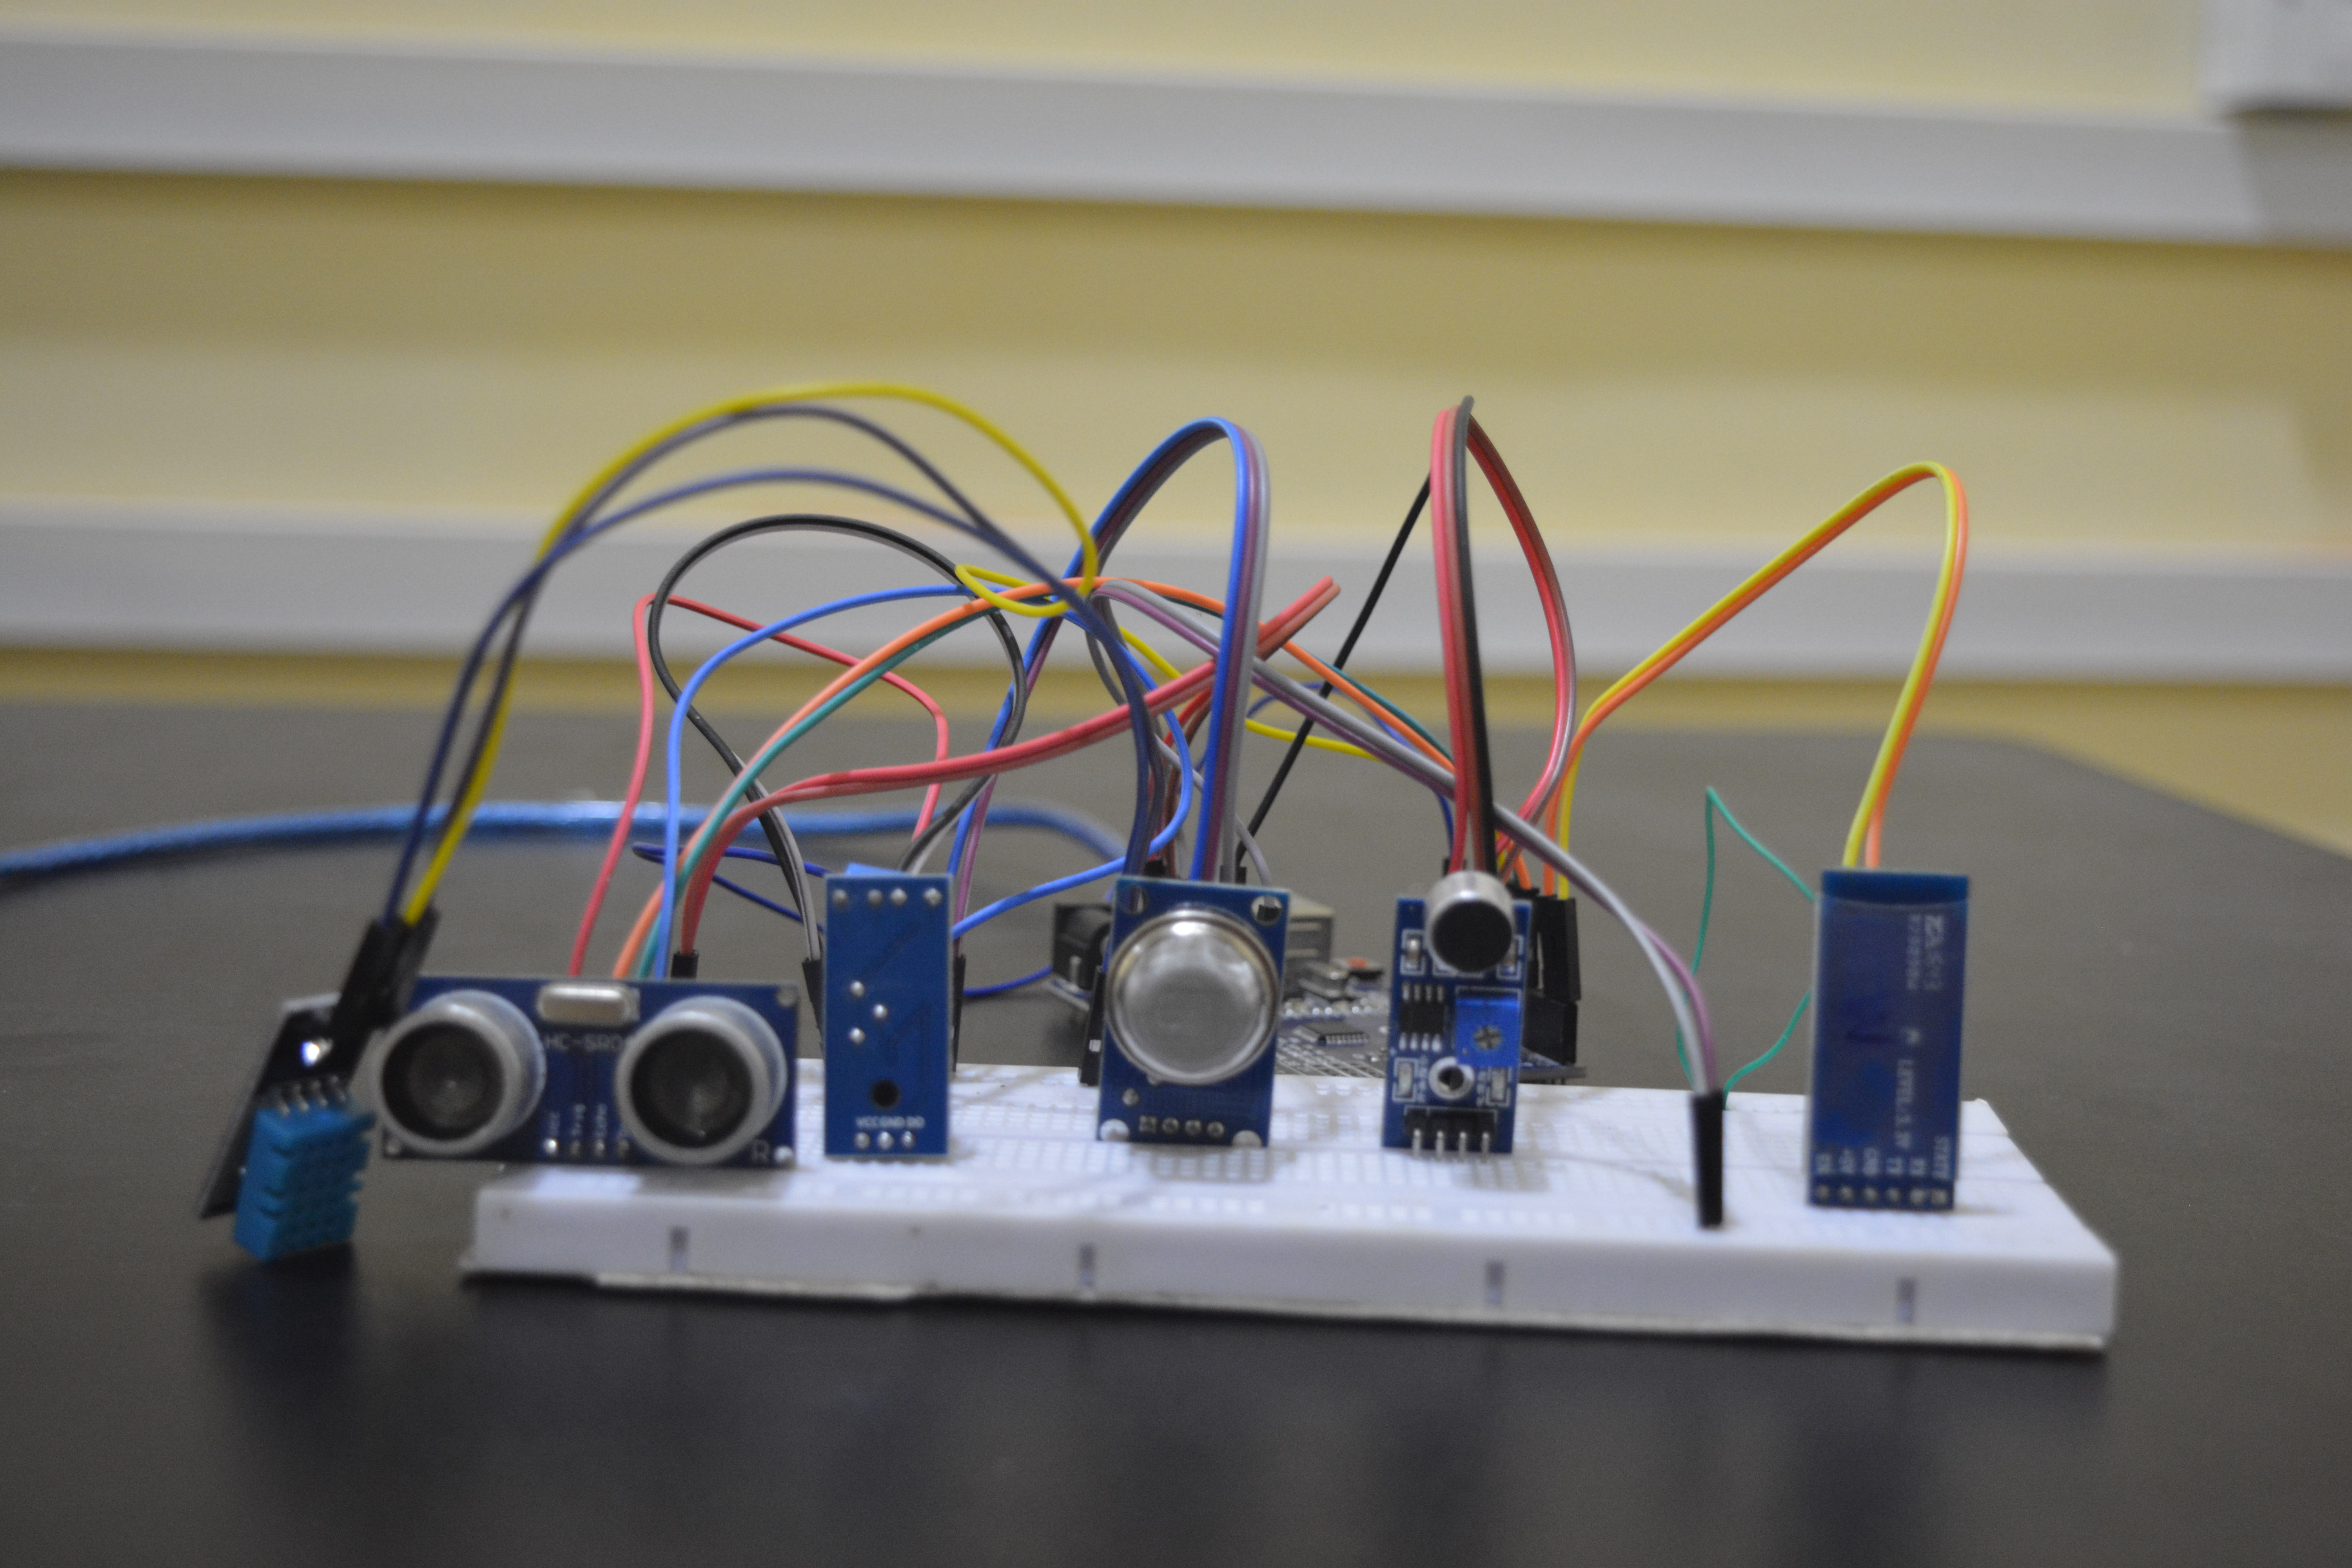
\includegraphics[width=4.0in]{master2}}
  \caption{ \textbf{}Master device }
  \end{figure}
\end{frame}
\begin{frame}\frametitle{Slave device circuit diagram}
  \begin{figure}[H]
  \centerline{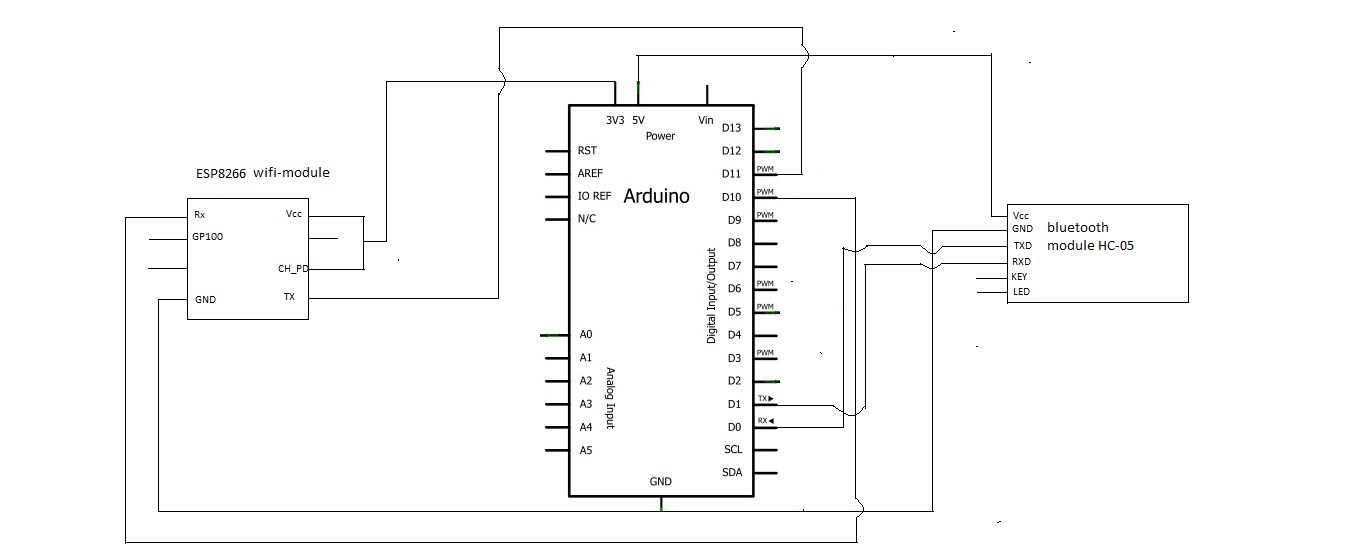
\includegraphics[width=4.0in]{SC.JPG}}
  \caption{ \textbf{}Slave device circuit diagram}
  \end{figure}
\end{frame}
\begin{frame}\frametitle{Slave device}
  \begin{figure}
  \centerline{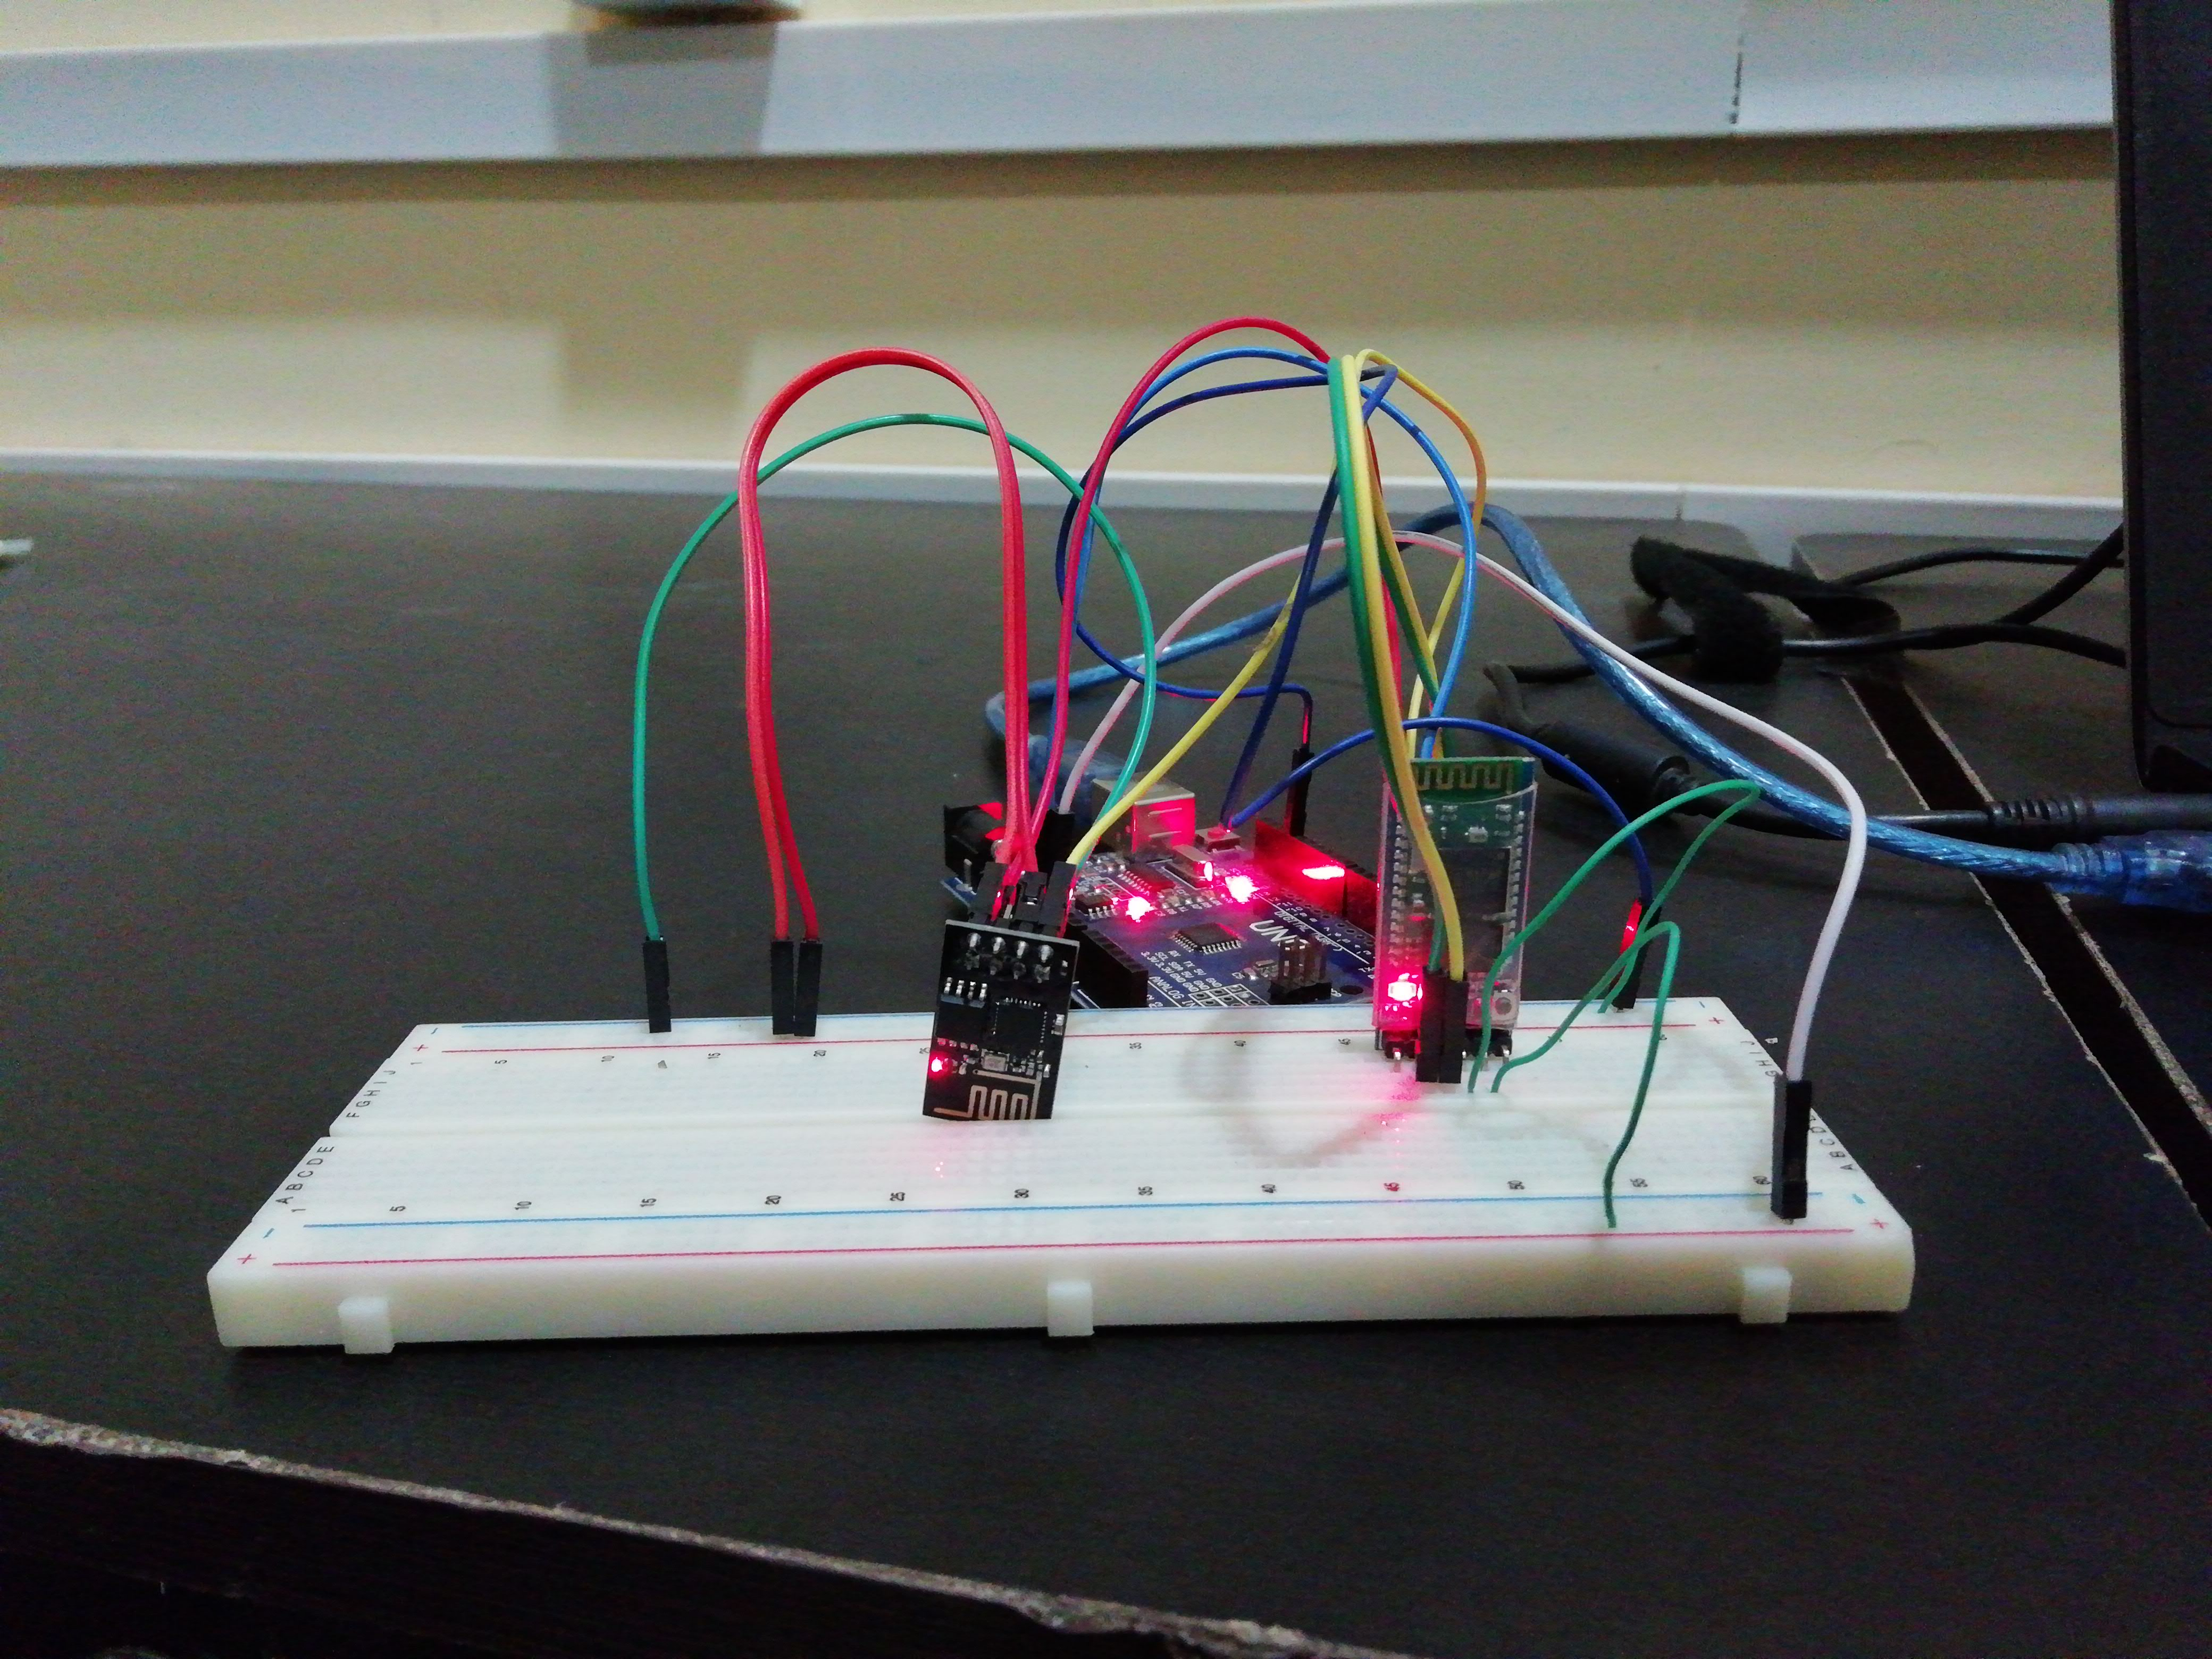
\includegraphics[width=4.0in]{sl.jpg}}
  \caption{ \textbf{}Slave device transfer data to the cloud}
  \end{figure}
\end{frame}
\begin{frame}\frametitle{Data communication between two Bluetooth modules }
\begin{itemize}
\item Bluetooth module is used to communicate between master and slave device.
\item A master Bluetooth module is connected to master device to send data to the slave device. 
\item A slave Bluetooth module is connected to slave device to receive data from the master device.
\item Bluetooth modules used serial port protocol for communication between two device.
\end{itemize}
\end{frame}

\begin{frame}\frametitle{Data transmission to cloud and fault analysis}
\item Data transmission to cloud
\begin{itemize}
\item ESP2866 WI-FI module is used to send sensor data into cloud.
\item We had used Think-Speak cloud to save our sensor data.  
\end{itemize}
\item Fault analysis
\begin{itemize}
\item The collected data in the cloud is used for fault analysis.
\end{itemize}
\end{frame}
\begin{frame}\frametitle{Testing}
\begin{itemize}
\item We have tested few sensors on different environments.
\item We also tested our device with different configuration.  
\end{itemize}
\end{frame}
\begin{frame}
\begin{itemize}\frametitle{Results}
\item We have integrated five sensors on a single micro controller for effective reliability. 
\item We have established a wireless communication between two devices.
\item We have used different configuration of sensors for different environments.
\item The collected data in a cloud storage is used for fault diagnosis.
\item A threshold value is calculated by fault diagnosis.
\item The operator receives a message if variations in sensor data exceed threshold value. 
\end{itemize} 
\end{frame}
\begin{frame}
\begin{itemize}
\item Data representation for ultrasonic sensor and sound sensor in cloud.
  \begin{figure}[H]
  \centerline{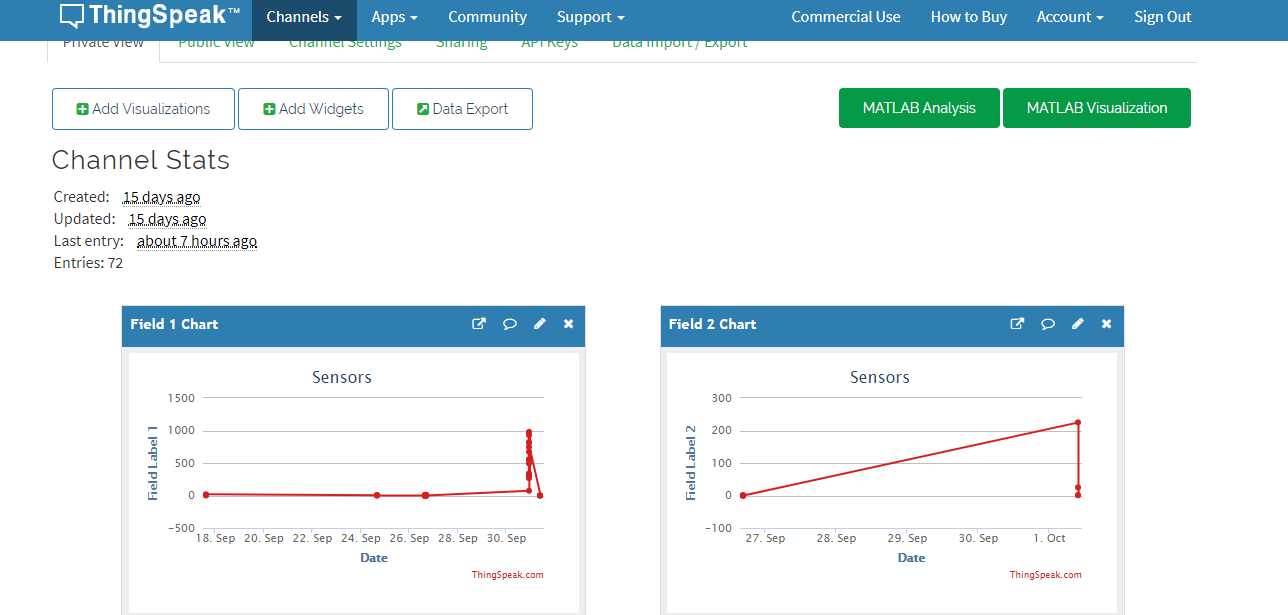
\includegraphics[width=4.0in]{01.JPG}}
  \caption{ \textbf{}Data representation in cloud for two sensors}
  \end{figure}
\end{itemize}
\end{frame}
\begin{frame}
\begin{itemize}
\item Data representation for multiple sensors in cloud.
  \begin{figure}
  \centerline{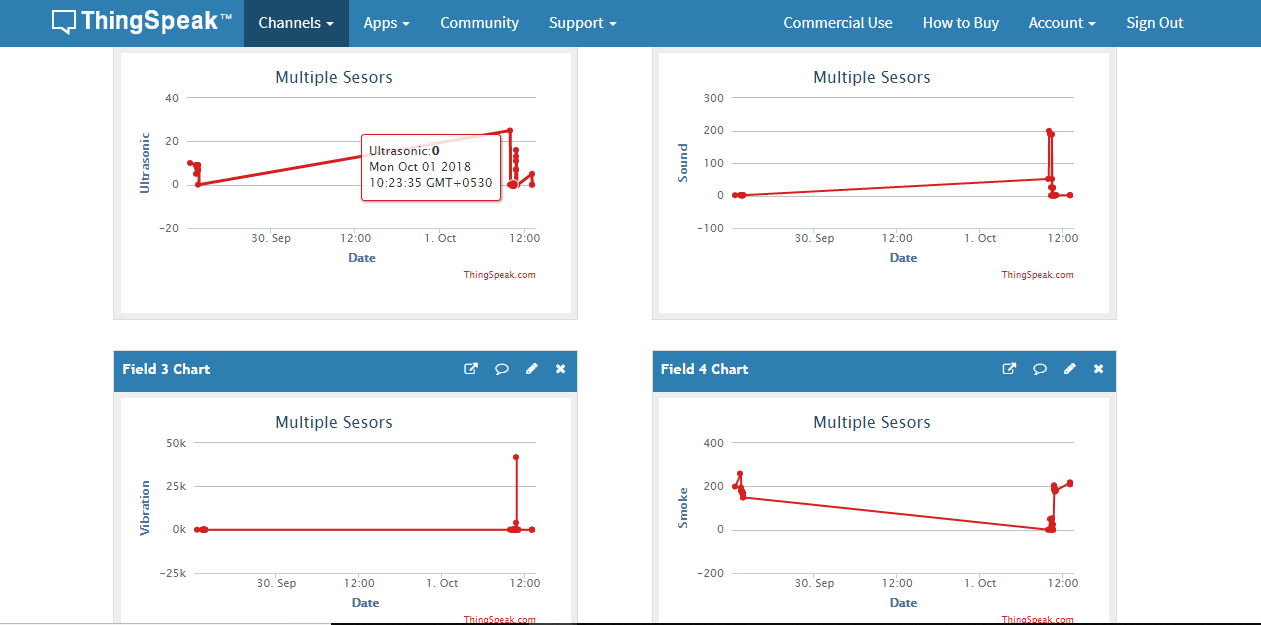
\includegraphics[width=4.0in]{22.JPG}}
  \caption{ \textbf{}Data representation in cloud for multiple sensors}
  \end{figure}
\end{itemize}
\end{frame}

\begin{frame}\frametitle{Conclusion}
\item 
\begin{itemize}
    
\end{itemize}
\begin{itemize}
\item Our main prospect of the project dealing with making an low cost IoT application which can become useful for the many industrial process and in their maintenance prospects.
\item 
Important factor which our objective results is in decreasing the employee engagement and automation  which help companies to shape up economically.
\item It can also help to increase productivity 
\end{itemize}
\end{frame}
\begin{frame}\frametitle{Future Work}
Future work may comprise
\begin{itemize}
\item As a future work we will test our project in the large scale industries.
\item We will develop a mathematical model to identify a threshold value for better health monitoring of industrial machines.
\end{itemize}
\end{frame}
\begin{frame}\frametitle{References}
\begin{itemize}
\printbibliography
\end{itemize}
\end{frame}
\begin{frame}
\Huge
\begin{center}Thank You \end{center}
\end{frame}
\end{document}